\section*{Results}

%%%%%%%%%%%%%%%%%%%%%%%%%%%%%%%%%%%%%%%%%%%%%%%%%%%%%%%%%%%%
\renewcommand{\arraystretch}{1.1}
\begin{table}[tb]

\begin{center}
 \caption[]{$F_{ST}$ of synonymous and noncoding GBS SNPs}
  \textbf{}\\[-2mm]
{\fontsize{6}{9}\sf
    \begin{tabular}{llccccccl}
    \hline
    & & \\[-3mm]
	&		&	\multicolumn{2}{c}{Mesoamerica}		&	\multicolumn{2}{c}{S. America}		\\
	&		&	Lowlands	&	Highlands	&	Lowlands	&	Highlands	\\
      \hline
    & & \\[-3mm]
Mesoamerica	&	Lowlands	&	--		&			&			&		\\
		&	Highlands	&	0.0244	&	--		&			&		\\
S. America		&	Lowlands	&	0.0227	&	0.0343	&	--		&		\\
		&	Highlands	&	0.0466	&	0.0534	&	0.0442	&	--	\\ [1mm]
    \hline
    \end{tabular}
    \label{FstP}  % caption is needed to make this work
}
\end{center}
\end{table}
\renewcommand{\arraystretch}{1}
%%%%%%%%%%%%%%%%%%%%%%%%%%%%%%%%%%%%%%%%%%%%%%%%%%%%%%%%%%%%

 %%%%%%%%%%%%%%%%%%%%%%%%%%%%%%%%%%%%%%%%%%%%%%%%%%%%%%%%%%%%
\renewcommand{\arraystretch}{1.1}
\begin{table}[tb]

\begin{center}
 \caption[]{Estimated parameters of population size model}
  \textbf{}\\[-2mm]
{\fontsize{7}{11}\sf
    \begin{tabular}{lcccccccl} \hline
       & & \\[-3mm]
     Mesoamerica  & \multicolumn{2}{c}{Model IA}  &\multicolumn{2}{c}{Model IB}\\[0.1cm]
    \hline
    & & \\[-3mm]
   & Likelihood   & $-$5592.80 & Likelihood       &  $-$4654.79 \\
   &$N_C$      &  138,000             & $N_C$        & 225,000 \\
   &$N_1$        & 52,440             & $N_1$          & 171,000\\ 
   &$N_2$        & 85,560             & $N_2$          & 54,000\\    
   &$N_{2P}$   & 85,560                   &  $N_{2P}$   & 54,000\\ 
      \hline
    & & \\[-3mm]
    S. America  & \multicolumn{2}{c}{Model IA}  &\multicolumn{2}{c}{Model II}\\[0.1cm]
        \hline
     & & \\[-3mm]
      & Likelihood   &  $-$3855.28 & Likelihood     &  $-$8044.71 \\
      &$N_C$      & 78,000              & $N_C$       & 150,000 \\
      &$N_1$        & 75,660             & $N_1$      & 96,000\\ 
      &$N_2$        & 2,340               & $N_2$      & 54,000\\      
      &$N_{2P}$   & 205,920        &  $N_3$     & 51,300\\
      &                   &                         &  $N_4$     & 2,700\\      
      &                    &                     &  $N_{4P}$    & 145,800\\ [1mm]
    \hline
%    \multicolumn{9}{l}{$^{a}$ The groups were based on phylogenetic analysis in fig.~\ref{tree}\emph{A}}\\
    \end{tabular}
    \label{param}  % caption is needed to make this work
}
\end{center}
\end{table}
\renewcommand{\arraystretch}{1}
%%%%%%%%%%%%%%%%%%%%%%%%%%%%%%%%%%%%%%%%%%%%%%%%%%%%%%%%%%%%


\subsection*{Samples and data}

We sampled 94 maize landraces from four distinct regions in the Americas (Table \ref{srkid}): the lowlands of Mesoamerica (Mexico/Guatemala; $n=24$) and northern S. America ($n=23$) and the highlands of Mesoamerica ($n=24$) and the Andes ($n=23$). 
Samples were genotyped using the MaizeSNP50 Beadchip platform (``MaizeSNP50''; $n=94$) and genotyping-by-sequencing (``GBS''; $n=87$). 
After filtering for Hardy-Weinberg genotype frequencies and minimum sample size at least 10 in each of the four populations (see Materials and Methods) 91,779 SNPs remained, including 67,828 and 23,951 SNPs from GBS and MaizeSNP50 respectively.  

\subsection*{Population structure}

We performed a {\sf STRUCTURE} analysis \cite[]{Pritchard_2000_10835412,Falush_2003_12930761} of our landrace samples, varying the number of groups from $K$ = 2 to 6 (Figure~\ref{map}, Figure~\ref{supp:struct}). 
Most landraces were assigned to groups consistent with \emph{a priori} population definitions, but admixture between highland and lowland populations was evident at intermediate elevations ($\sim1700$m).  Consistent with previously described scenarios for maize diffusion \cite[]{Piperno_2006_69}, we find evidence of shared ancestry between lowland Mesoamerican maize and both Mesoamerican highland and S. American lowland populations.  Pairwise $F_{ST}$ among populations reveals low overall differentiation (Table \ref{FstP}), and the higher $F_{ST}$ values observed in S. America are consistent with the decreased admixture seen in {\sf STRUCTURE}.  Archaeological evidence supports a more recent colonization of the highlands in S. America  \cite[]{Piperno_2006_69,Perry_2006_16511492,Grobman_2012_22307642}, suggesting that the observed differentiation may be the result of a stronger bottleneck during colonization of the S. American highlands.  

%%%%%%%%%%%%%%%%%%%%%%%%%%%%%%%%%%%%%%%%%% FIGURE
\begin{figure}[tb]   
  \begin{center}
   \vspace{-0mm}
   %\includegraphics[width=0.23\textwidth]{figs/model}
   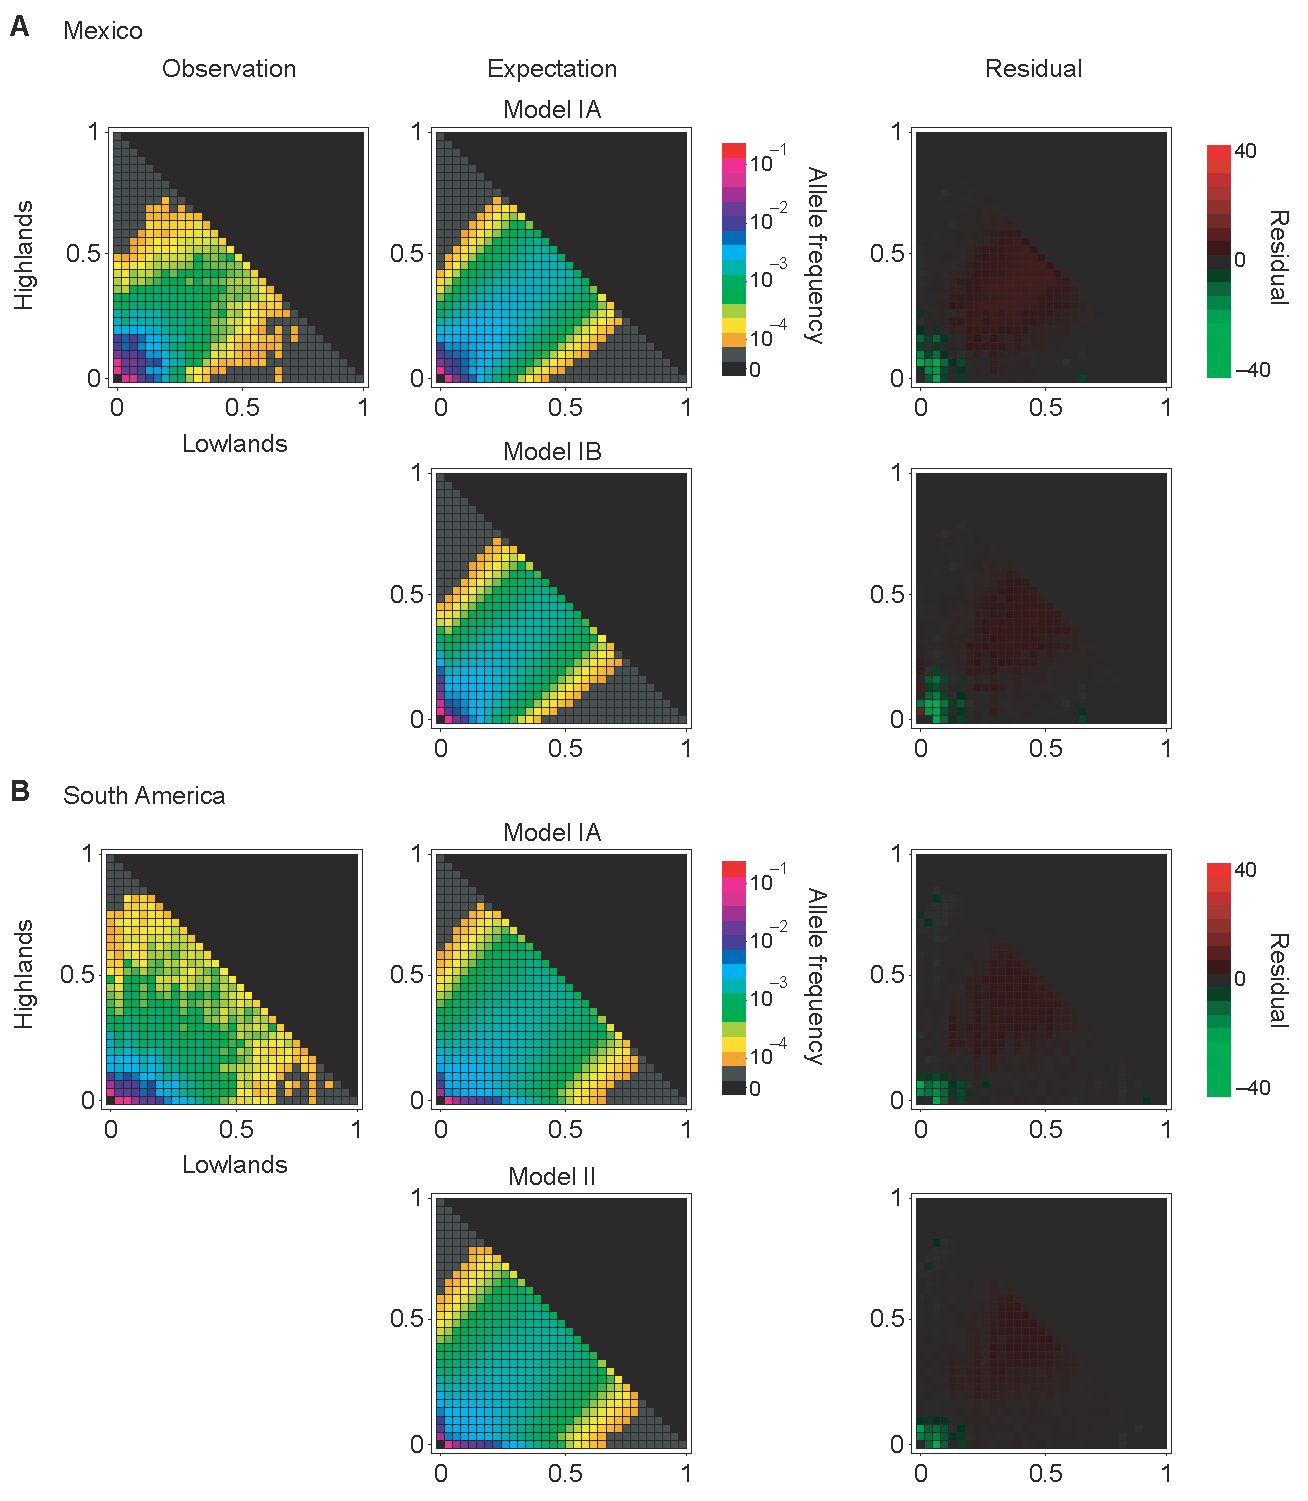
\includegraphics[width=0.5\textwidth]{fig/Fig4}
   \renewcommand{\baselinestretch}{0.9}
   \vspace{-3mm}
   \caption{Observed and expected joint distributions of minor allele frequencies in lowland and highland populations in (A) Mesoamerica and (B) S. America. Residuals are calculated as  $(\mbox{model}-\mbox{data})/\sqrt[]{\mbox{model}}$}.
\vspace{-6mm}
    \label{JFD}
  \end{center}
\end{figure}
%%%%%%%%%%%%%%%%%%%%%%%%%%%%%%%%%%%%%%%%%% FIGURE

\subsection*{Population differentiation}

To provide a null expectation for allele frequency differentiation, we used the joint site frequency distribution (JFD) of lowland and highland populations to estimate parameters of two demographic models  using the maximum likelihood method implemented in $\delta a \delta i$ \cite[]{Gutenkunst_2009_19851460}.  
All models incorporate a domestication bottleneck \cite[]{Wright_2005_15919994} and population differentiation between lowland and highland populations, but differ in their consideration of admixture and ascertainment bias (Figure~\ref{model}; see Materials and Methods for details).

Estimated parameter values are listed in Figure~\ref{model} and Table~\ref{param}; while the observed and expected JFDs were quite similar for both models,  residuals indicated an excess of rare variants in the observed JFDs in all cases (Figure~\ref{JFD}). 
Under both models IA and IB,  we found expansion in the highland population in Mesoamerica to be unlikely, but a strong bottleneck followed by population expansion is supported in S. American highland maize in both models IA and II.  
The likelihood value of model IB was higher than the likelihood of model IA by 850 units of log-likelihood (Table~\ref{param}), consistent with analyses suggesting that introgression from \textit{mexicana} played a significant role during the spread of maize into the Mesoamerican highlands \cite[]{Profford_2013}. 

In addition to the parameters listed in Figure~\ref{model}, we investigated the impact of varying the domestication bottleneck size ($N_B$).  
Surprisingly, $N_B$ was estimated to be equal to $N_C$, the population size at the end of the bottleneck, and the likelihood of $N_B<N_C$ was much smaller than for alternative parameterizations (Table~\ref{param} and Table~\ref{supp:param}). 

Comparisons of our empirical $F_{ST}$ values to the null expectation simulated under our demographic models allowed us to identify significantly differentiated SNPs between lowland and highland populations. In all cases, observed $F_{ST}$ values were quite similar to those generated under our null models (Figure~\ref{FstDist}), and model choice -- including the parameterization of the domestication bottleneck -- had little impact on the distribution of estimated \emph{P}-values (Figure~\ref{fig:qq}). 
We show results under Model IB for Mesoamerican populations and Model II for S. American populations.
We chose $P<0.01$ as an arbitrary cut-off for significant differentiation between lowland and highland populations, and identified 687 SNPs in Mesoamerica (687/76,989=0.89\%) and 409 SNPs in S. America (409/63,160=0.65\%) as significant outliers (Figure~\ref{PvDist}). Different cutoff values (0.05, 0.001) gave qualitatively identical results (data not shown). SNPs with significant $F_{ST}$ $P$-values were enriched in intergenic regions rather than protein coding regions (60.0\% vs. 47.9\%, Fisher's Exact Test $P < 10^{-7}$ for Mesoamerica; 62.0\% vs. 47.8\%, FET $P<10^{-5}$ for S. America).
Different cutoff values (0.05, 0.001) gave qualitatively identical results (data not shown).
%\jri{ fix "data not shown" if going to PLoS Gen.}

%%%%%%%%%%%%%%%%%%%%%%%%%%%%%%%%%%%%%%%%%% FIGURE
\begin{figure}[tb]   
  \begin{center}
   \vspace{-0mm}
   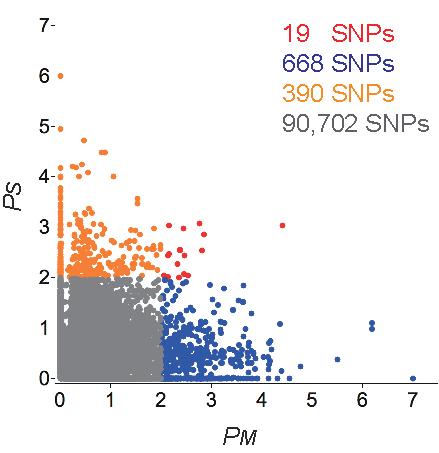
\includegraphics[width=0.4\textwidth]{fig/Fig6}
   \renewcommand{\baselinestretch}{0.9}
   \vspace{-3mm}
   \caption{Scatter plot of $-\log_{10} P$-values of observed $F_{ST}$ values based on simulation from estimated demographic models. $P$-values are shown for each SNP in both Mesoamerica (Model IB; $P_M$ on $x$-axis) and S. America (Model II; $P_S$ on $y$-axis).  
   Red, blue, orange and gray dots represents SNPs showing significance in both Mesoamerica and S. America, only in Mesoamerica, only in S. America, or in neither region, respectively (see text for details).
   The number of SNPs in each category is shown in the same color as the points.} 
\vspace{-6mm}
    \label{PvDist}
  \end{center}
\end{figure}
%%%%%%%%%%%%%%%%%%%%%%%%%%%%%%%%%%%%%%%%%% FIGURE

\subsection*{Patterns of adaptation}

Given the historical spread of maize from an origin in the lowlands, it is tempting to assume that the observation of significant population differentiation at a SNP should be primarily due to an increase in frequency of adaptive alleles in the highlands.
To test this hypothesis, we sought to identify the adaptive allele at each locus using comparisons between Mesoamerica and S. America as well as to \emph{parviglumis}. 
Alleles were called ancestral if they were at higher frequency in \emph{parviglumis}, or uncalled in \emph{parviglumis} but at higher frequency in all populations but one. 
SNPs were consistent with Mesoamerica-specific adaptation if one allele was at high frequency in one Mesoamerican population, low frequency in the other Mesoamerican population, and either: low frequency in \emph{parviglumis} and at most intermediate frequency in S. American populations, or missing in \emph{parviglumis} and at low frequency in S. American populations.
On the other hand, SNPs were consistent with adaptation to highlands in both regions if they were at high frequency in both highland populations, and at low frequency in the lowland populations and \emph{parviglumis}; and vice-versa for adaptation to lowlands in both regions.
SNPs with an allele at high frequency in one highland and the alternate lowland population are suggestive of adaptation in both populations but on different haplotypes created by recombination.

Consistent with predictions, we infer that differentiation at 72.3\% (264) and 76.7\% (230) of SNPs in Mesoamerica and S. America is due to adaptation in the highlands after excluding  SNPs with ambiguous patterns likely due to recombination. 
The majority of these SNPs show patterns of haplotype variation (by the PHS test) consistent with our inference of selection (Table~\ref{supp:phs} and Supporting Information, File S1).
   
Convergent evolution at the nucleotide level should be reflected in an excess of SNPs showing significant differentiation between lowland and highland populations in both Mesoamerica and S. America. 
Although the 19 SNPs showing $F_{ST}$ \emph{P}-values  $<0.01$ in both Mesoamerica ($P_M$) and S. America ($P_S$) is statistically greater than the $\approx 5$ expected ($48,370\times 0.01 \times 0.01 \approx 4.8$; $\chi^2$-test, $P\ll0.001$), it nonetheless represents a small fraction ($\approx 7-8\%$) of all SNPs showing evidence of selection.
This paucity of shared selected SNPs does not appear to be due to our demographic model: 
a simple outlier approach based using the 1\% highest $F_{ST}$ values finds no shared adaptive SNPs between Mesoamerican and S. American highland populations. 
For 13 of 19 SNPs showing putative evidence of shared selection we could use data from \textit{parviglumis} to infer whether these SNPs were likely selected in lowland or highland conditions (Supporting Information, File S1).  
Surprisingly, SNPs identified as shared adaptive variants more frequently showed segregation patterns consistent with lowland  (10 SNPs) rather than highland adaptation (2 SNPs). %(1 SNP with an ambiguous pattern). 

We also investigated how often different SNPs in the same gene may have been targeted by selection. 
To search for this pattern, we considered all SNPs within 10kb of a transcript as part of the same gene, though SNPs in an miRNA or second transcript within 10kb of the transcript of interest were excluded.  
We classified SNPs showing significant $F_{ST}$ in Mesoamerica, S. America or in both regions into 778 genes. 
Of these, 485 and 277 genes showed Mesoamerica-specific and SA-specific significant SNPs, while 14 genes contained at least one SNP with a pattern of differentiation suggesting convergent evolution and 2 genes contained both Mesoamerica-specific and SA-specific significant SNPs. 
Overall, however, fewer genes showed evidence of convergent evolution than expected by chance (permutation test; $P<10^{-5}$). 
Despite similar phenotypes and environments, we thus see little evidence for convergent evolution at either the SNP or the gene level.  

\subsection*{Comparison to theory}

% # \mutrate computation:
% A <- 500; rho <- 5000; sb <- 10^(-(1:4)); xisq <- 30
% sapply( 10^c(-5,-8), function (mu) mu * (2 * rho * A * sb)/xisq )

Given the limited empirical evidence for convergent evolution at the molecular level, we took advantage of recent theoretical efforts \cite[]{ralph2014convergent} to assess the degree of convergence expected under a spatially explicit population genetic model (see Materials and Methods).
Our modeling estimates assume a maize population density $\rho$ of the highlands to be around (0.5 ha field/person) $\times$ (0.5 people/km$^2$) $\times$ ($2\times 10^4$ plants per ha field) $=$ 5,000 plants per km$^2$.
The area of the Andean highlands currently under maize cultivation is estimated to be approximately $A=8400\text{km}^2$, giving a total maize population of $A \rho = 4.2 \times 10^7$. 
Assuming an offspring variance of $\xi^2 = 30$, we can then compute the waiting time $\Tmut=1/\mutrate$ for a new beneficial mutation to appear and fix.
We observe that even if there is relatively strong selection for an allele at high elevation ($s_b=0.01$), a single-base mutation with mutation rate $\mu=10^{-8}$ would take an expected 3,571 generations to appear and fix.
Our estimate of the maize population size uses the land area currently under cultivation and is likely an overestimate; $\Tmut$ scales linearly with the population size and lower estimates of $A$ will thus increase $\Tmut$ proportionally.
However, because $\Tmut$ also scales approximately linearly with both the selection coefficient and the mutation rate, strong selection and the existence of multiple equivalent mutable sites could reduce this time. 
For example, if any one of 10 sites within a gene could have equivalent strong selective benefit ($s_b=0.1$), $\Tmut$ would be reduced to 36 generations assuming constant $A$ over time. 

% # Tmig computation:
% A <- 500; rho <- 5000; xisq <- 30; sigma <- 3.5
% params <- expand.grid( R=1000*(1:4), sm=10^(-(1:4)) )
% params$char.length <- with(params, 1/(sqrt(2*sm)/sigma) )
% params$Tmig <- with( params, 1 / ( sm * (A * rho / 2) *  exp(- sqrt(2*sm)*R/sigma ) ) )
% print(params)

Gene flow between highland regions could also generate patterns of shared adaptive SNPs.
From our demographic model we have estimated a mean dispersal distance of $\sigma \approx 1.8$ kilometers per generation.
With selection against the highland allele in low elevations $10^{-1} \ge s_m \ge 10^{-4}$, 
the distance $\sigma/\sqrt{2s_m}$ over which the frequency of a highland-adaptive, lowland-deleterious allele decays into the lowlands is still short: 
between 7 and 250 kilometers.
Since the Mesoamerican and Andean highlands are around 4,000 km apart, the time needed for a rare allele with weak selective cost $s_m=10^{-4}$ in the lowlands 
to transit between the two highland regions is $\Tmig \approx 8 \times 10^{4}$ generations. 
While the exponential dependence on distance in equation \eqref{eqn:migrate} means that shorter distances could be transited more quickly, the waiting time $\Tmig$ is also strongly dependent on the magnitude of the deleterious selection coefficient: with $s_m=10^{-4}$, $\Tmig \approx 25$ generations over a distance of 2,000 km, but increases to $\approx 10^{8}$ generations with a still weak selective cost of $s_m=10^{-3}$.
%, however: with the still weak selective cost of $s_m=10^{-3}$, for example, $\Tmig$ is $10^8$ generations over 2,000km,
%-- if the distance between highland patches is 2,000 km (or if $\sigma$ is twice as large) then $\Tmig \approx 25$ generations, indicating that all alleles beneficial in both highlands but with such weak selection cost in the lowlands should be shared if they arose long enough ago for migration-selection balance to have been reached.
%and much larger for longer distances.

%\plr{The above has changed because I found an factor of 2 missed out in $\sigma$, 
%and the R code has an factor of $2s_b/\xi^2$ that wasn't present in \eqref{eqn:migrate}.
%This is an overestimate of the rate that is more correctly given in the supplement;
%I didn't worry about this before, when migration was unlikely for all parameter values.
%However, now $\Tmig$ is smallish for $R=1,000$ and $s_m=10^{-3}$ with the approximation \eqref{eqn:migrate},
%but not with the better expression of the appendix.
%This makes me want to put in the better expression, which I can't quickly motivate,
%except that the next bit makes it not matter, I think.}

However, the rough calculations with coalescent theory above show that even neutral alleles are not expected to transit between the Mesoamerican and Andean highlands within 4,000 generations.
This puts a lower bound on the time for deleterious alleles to transit as well, suggesting that we should not expect even weakly deleterious alleles (e.g.\ $s_m=10^{-4}$) to have moved between highlands.

Taken together, these theoretical considerations suggest that any alleles beneficial in the highlands that are neutral or deleterious in the lowlands that are shared by both the Mesoamerican and S. American highlands would have been present as standing variation in both populations, rather than passed between them.


\subsection*{Alternative routes of adaptation}
The lack of both empirical and theoretical support for convergent adaptation at SNPs or genes led us to investigate alternative patterns of adaptation. 

We first sought to understand whether SNPs showing high differentiation between the lowlands and the highlands arose primarily via new mutations or were selected from standing genetic variation.  
We found that putatively adaptive variants identified in both Mesoamerica and S. America tended to segregate in the lowland population more often than other SNPs of similar mean allele frequency (85.3\% vs. 74.8\% in Mesoamerica (Fisher's exact test $P < 10^{-9}$ and 94.8\% vs 87.4\% in S. America,  $P< 10^{-4}$).  
We extended this analysis by retrieving SNP data from 14 \emph{parviglumis} inbred lines included in the Hapmap v2 data set, using only SNPs with $n\geq10$ \cite[]{Chia_2012_22660545,Hufford_2012_22660546}.  
Again we found that putatively adaptive variants were more likely to be polymorphic in \emph{parviglumis} (78.3\% vs. 72.2\% in Mesoamerica 
(Fisher's exact test $P < 0.01$ and 80.2\% vs 72.8\% in S. America,  $P< 0.01$). 

While maize in highland Mesoamerica grows in sympatry with the highland teosinte \textit{mexicana}, maize in S. America is outside the range of wild \textit{Zea} species, leading to a marked difference in the potential for adaptive introgression from wild relatives.
\citet{Pyhajarvi2013} recently investigated local adaptation in \textit{parviglumis} and \textit{mexicana} populations, characterizing differentiation between these subspecies using an outlier approach.
Genome-wide, only a small proportion (2--7\%) of our putatively adaptive SNPs were identified by \citet{Pyhajarvi2013}, though these numbers are still in excess of expectations (Fisher's exact test $P<10^{-3}$ for S. America and $P<10^{-8}$ for Mesoamerica; Table~\ref{tanja}).
The proportion of putatively adaptive SNPs shared with teosinte was twice as high in Mesoamerica, however, 
leading us to evaluate the contribution of introgression  from \textit{mexicana} \cite[]{Profford_2013} in patterning differences between S. American and Mesoamerican highlands.  

The proportion of putatively adaptive SNPs in introgressed regions of the genome in highland maize in Mesoamerica was nearly four times higher than found in S. America (FET $P<10^{-11}$), while differences outside introgressed regions were much smaller (7.5\% vs. 6.2\%; Table \ref{supp:introgressed}). 
Furthermore, of the 77 regions identified as introgressed in \cite{Profford_2013}, more than twice as many contain at least one $F_{ST}$ outlier in Mesoamerica as in S. America (23 compared to 9, one-tailed Z-test $P=0.0027$).
Excluding  putatively adaptive SNPs, mean $F_{ST}$ between Mesoamerica and S. America is only slightly higher in introgressed regions (0.032) than across the rest of the genome (0.020), suggesting the enrichment of high $F_{ST}$ SNPs seen in Mesoamerica is not simply due to neutral introgression of a divergent teosinte haplotype.  
%\ref{supp:introgressed}


%When focusing on GUs, we identified 99/586 (14.5\%) and 22/466 (4.7\%) GUs of Mesoamerica- and SA-specific significance in introgressed regions (Fisher's exact test, $P<10^{-6}$). 


    
